\documentclass{article}

% Language setting
% Replace `english' with e.g. `spanish' to change the document language
\usepackage[english]{babel}

% Custom packages
\usepackage{color,soul} % For highlighting text
\usepackage{float} % For controlling figure placement ([H] option)
\usepackage{amsmath}
\usepackage{amssymb} % For mathematical symbols such as \lessgtr
\DeclareMathOperator*{\argmax}{arg\,max}
\DeclareMathOperator*{\argmin}{arg\,min}

% Set page size and margins
% Replace `letterpaper' with `a4paper' for UK/EU standard size
\usepackage[letterpaper,top=2cm,bottom=2cm,left=3cm,right=3cm,marginparwidth=1.75cm]{geometry}

% Useful packages
\usepackage{graphicx}
\usepackage[colorlinks=true, allcolors=blue]{hyperref}

\definecolor{mulberry}{rgb}{0.77, 0.29, 0.55}
\newcommand{\dm}[1]{{\color{mulberry} #1}}

\newcommand{\mi}{\mathrm{i}}

\title{Statistical analysis of Kernel-Nulling output distributions for high contrast detection of exoplanets in VLTI and LIFE configurations}

\author{Vincent Foriel,
        David Mary,
        Frantz Martinache
       }

\begin{document}

\maketitle

\begin{abstract}
Kernel-nulling interferometry represents a promising approach for direct exoplanet detection. This technique generates characteristic kernel-null depth distributions depending on the presence or absence of a planetary companion. Statistical analysis of these distributions is essential for robust planet detection. We develop and compare several statistical tests to efficiently discriminate between the ${\mathcal{H}}_0$ (star-only) and ${\mathcal{H}}_1$ (star-planet system) hypotheses. We analyze the performance of different test statistics including mean, median, mode, Kolmogorov-Smirnov, Cramér-von Mises, and Wilcoxon-Mann-Whitney tests. We conduct numerical simulations for two instrumental scenarios: ground-based VLTI and space-based LIFE configurations. For each scenario, we generate datasets under both ${\mathcal{H}}_0$ and ${\mathcal{H}}_1$ hypotheses, accounting for specific instrumental parameters and noise levels. We evaluate test performance using ROC curves and P-value analysis. \hl{Ajouter les résultats quantitatifs obtenus}. This statistical analysis, currently applied to simulated data, paves the way for robust high-contrast exoplanet detection using kernel-nulling interferometry.
\end{abstract}

%------------------------------------------------------------------------------

\dm{OK résumé de mes coms détailles ci-dessous : le plus gros boulot à faire pour l'itération suivante c'est : \\
- en intro : biblio : recenser, comparer, contraster pour mettre en évidence l'originalité du papier\\
- en intro : justification de l'intérêt scientifique du papier (/exoplanètes, VLTI, LIFE) et de son scope (portée attendu des simus ?) \\
- Sec. 2 étude statistique plus poussée des différents régimes, types de distribution, influence des paramètres, classement et présentation des résultats pour justifier la section d'après (les tests mis en opuvre)\\
- Sec. 3 : La formalisation rigoureuse des tests, classement, formules analytiques \\
- Sec. 4 : Etude comparative des performances dans les résultats }

\section{Introduction}

Direct imaging of exoplanets remains one of the major challenges in modern astronomy, requiring techniques capable of overcoming contrast constraints (beyond $10^{-8}$ to allow exo-Earth detection) and angular separation requirements (on the order of milli-arcseconds). Nulling interferometry, initially proposed by \cite{Bracewell1979}, uses destructive interference to suppress stellar light while preserving the planetary signal, thus addressing both angular resolution and contrast challenges.

Kernel-Nulling \cite{Martinache2018} improves this approach by using four telescopes and phase-quadrature signals, enabling the creation of signal combinations (Kernel-Nulls) that are robust to first-order phase aberrations. This technique generates characteristic statistical distributions depending on the presence or absence of a planetary companion due to the interferometric nature of the measurements: when a companion is present, it introduces additional coherent flux that shifts the kernel-null depth distribution (Fig \ref{fig:distribution}). The shape and magnitude of this shift depend on the companion's contrast ratio, angular separation, and position angle relative to the stellar system.

\hl{Besoin d'expliquer plus en détail la Figure 1: pourquoi la distribution rouge est centrée sur zéro (star-only) et pas la bleue (avec compagnon)? Spécifier les paramètres exacts de simulation utilisés (contraste du compagnon, nombre de trames, erreurs de phase, etc.). Clarifier si c'est seulement un décalage ou si la forme de la distribution change aussi et pourquoi.}

However, these distributions do not follow standard probability laws (discussed in Sec. \ref{sec:distribution_analysis}), presenting unique challenges for statistical analysis. \hl{Préciser quelles sont les difficultés spécifiques: distributions inconnues a priori, mélanges de distributions, faibles différences à détecter pour des contrastes élevés, etc.}

\hl{Il manque une section bibliographie détaillée ici: recenser les méthodes existantes pour détecter des différences entre distributions dans le contexte exoplanètes et plus généralement en astronomie. Comparer et contraster pour mettre en évidence l'originalité de ce papier. Quelles différences entre les problématiques connexes trouvées et celle-ci?}

\hl{Il manque aussi une justification de l'intérêt scientifique: faire un topo sur VLTI et LIFE par rapport à la détection d'exoplanètes, décrire comment l'approche kernel-nulling se compare aux autres approches (pros/cons), quel est le statut des méthodes prévues actuellement, contraster par rapport aux travaux de Hanot \& co.}

Analysis of these distributions therefore requires dedicated statistical tools to efficiently discriminate between the two hypotheses: ${\mathcal{H}}_0$ (star-only) and ${\mathcal{H}}_1$ (star-planet system). In this work, we develop and compare several statistical tests to optimize exoplanet detection using Kernel-Nulling.

\hl{Ajouter le plan du papier ici}

\begin{figure}[H]
\centering
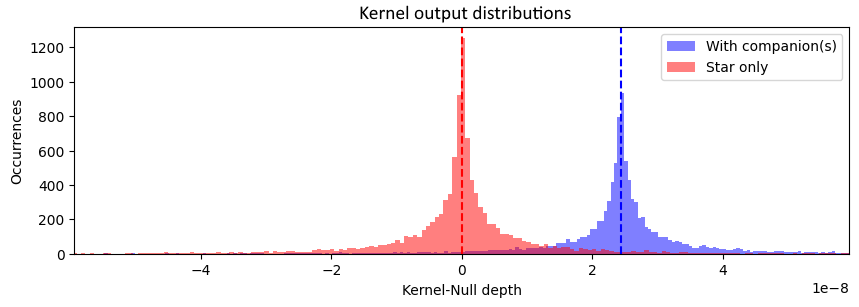
\includegraphics[width=\linewidth]{img/output_distribution.png}
\caption{Example of kernel-null depth distributions for ${\mathcal{H}}_0$ (star-only) and ${\mathcal{H}}_1$ (with companion) hypotheses. This example scenario is highly exaggerated with a companion contrast of \hl{[spécifier le contraste exact]} to induce a significant shift of the distribution. In practice, the two distributions are usually much closer and harder to distinguish, with typical contrast differences of \hl{[spécifier les valeurs typiques]}. \hl{Spécifier tous les paramètres de simulation: nombre de trames, erreurs de phase RMS, diamètre des télescopes, longueur d'onde, etc.}}
\label{fig:distribution}
\end{figure}

%--------------------------------------------------------------------

\section{Methodology}

\subsection{Data generation}

In this study, we consider two distinct instrumental scenarios for generating simulated data:

\begin{table}[H]
\centering
\begin{tabular}{|l|c|c|}
\hline
\textbf{Parameter} & \textbf{VLTI} & \textbf{LIFE} \\
\hline
Number of telescopes & 4 & 4 \\
Telescope diameter & 8 m & 2 m \\
Configuration & Irregular & Regular (rectangular) \\
Maximum baseline & 130 m & 600 m \\
Operating environment & Ground & Space \\
Wavelength & $1.55\mu$m & $4\mu$m \\
Cophasing error (RMS) & 100 nm & 1 nm \\
\hline
\end{tabular}
\caption{Instrumental parameters for the two scenarios considered in this study.}
\label{tab:scenarios}
\end{table}

The VLTI scenario represents a realistic ground-based interferometric configuration, utilizing the existing infrastructure of the Very Large Telescope Interferometer. This configuration features four 8-meter Unit Telescopes arranged in an irregular baseline geometry with maximum separations up to 130 meters. Operating at $1.55\mu$m in the near-infrared H-band, VLTI benefits from established adaptive optics systems but suffers from atmospheric turbulence effects that limit the achievable cophasing stability to approximately 100 nm RMS.

The LIFE scenario, in contrast, represents a next-generation space-based interferometer designed specifically for exoplanet characterization. This configuration employs four 2-meter telescopes arranged in a regular rectangular geometry with baselines extending up to 600 meters. Operating at $4\mu$m in the thermal infrared, LIFE benefits from the pristine space environment, enabling exceptional phase stability with cophasing errors as low as 1 nm RMS. This dramatic improvement in stability, combined with the longer operating wavelength, provides enhanced sensitivity to Earth-like exoplanets in their habitable zones.

\hl{Expliquer en détail cette table pour que le lecteur ait l'impression de voir les instruments et que les simulations correspondent à une réalité réaliste et des manipulations à portée de main.}

For each scenario, datasets are generated under both ${\mathcal{H}}_0$ (star-only) and ${\mathcal{H}}_1$ (star-planet system) hypotheses, accounting for specific instrumental parameters and noise levels for each case. The Kernel-Nulling operation is assumed to be ideal in terms of the mathematical combination of telescope signals, meaning that the theoretical kernel-null combinations are perfectly implemented without instrumental errors in the beam combination process.

\hl{Il faut prévoir un appendice où tu résumes le principe de kernel-nulling pour que le lecteur te suive. Expliquer ce que signifie faire une opération de kernel nulling en pratique, lister tous les défauts qui font que ça ne peut pas être idéal. Différencier une opération de kernel null idéale et l'absence de bruit à la fin. Bien expliquer ce que capturent tes simulations et les fluctuations qui créent les distributions montrées en Fig. 1.}

\subsection{Distribution analysis}  \label{sec:distribution_analysis}

Before attempting to discriminate between the ${\mathcal{H}}_0$ and ${\mathcal{H}}_1$ hypotheses, it is essential to conduct a comprehensive analysis of the obtained distributions to identify characteristics that might facilitate their statistical analysis. This analysis encompasses the study of distribution shapes, symmetry properties, parameter dependencies, and the identification of different statistical regimes.

\hl{Cette section doit présenter une analyse détaillée des distributions: montrer comment les variations combinées de tous les paramètres importants mènent à des distributions différentes. Identifier et montrer tous les différents régimes de paramètres menant à des familles de distributions différentes. Lister tous les paramètres qui vont entrer en compte dans les performances de détection: contraste et position du compagnon, longueur d'onde, nombre de trames, puissance des erreurs de phase, diamètre des télescopes, etc. Faire une table de ces paramètres. Il faut être exhaustif dans l'analyse et faire une synthèse quantifiée qui reflète clairement tous les cas pour le lecteur.}

We compare simulated distributions to different standard probability laws, notably observing their symmetry and general shape. Among the tested laws, the Cauchy distribution appears to provide a relatively satisfactory fit (Fig. \ref{fig:fits}), although imperfect, especially in the distribution tails when the number of samples is high.

\hl{Cette conclusion doit être étayée par une analyse quantifiée. La figure 2 ne semble pas confirmer que le fit Cauchy soit satisfaisant comme mentionné.}

This observation suggests that the distributions exhibit heavy-tailed behavior, which has important implications for the choice of appropriate statistical tests. Heavy-tailed distributions are particularly challenging for mean-based statistics, as they are sensitive to outliers, and favor robust statistical approaches.

\hl{Justifier théoriquement et/ou empiriquement (via l'optique et les simulations) si les distributions doivent être symétriques. Ajouter éventuellement des acquisitions de données sur banc pour appuyer ces hypothèses.}

\begin{figure}[H]
\centering
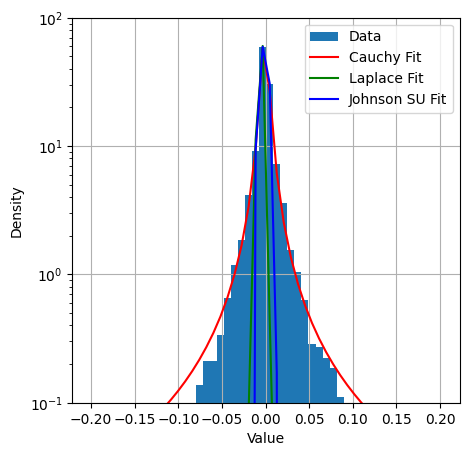
\includegraphics[width=6cm]{img/fits.png}
\caption{Fitting of standard probability laws to simulated distributions. The Fitter python package was used to perform the fitting of most of the usual laws. This figure shows the fit of the three most relevant laws the package identified. \hl{Ajouter une analyse quantitative de la qualité des fits, par exemple avec des métriques comme le test de Kolmogorov-Smirnov ou Anderson-Darling.}}
\label{fig:fits}
\end{figure}

\subsection{Statistical tests implemented}

Our statistical approach is motivated by the observed characteristics of kernel-null depth distributions. Given that we primarily expect distribution shifts when a companion is present, we logically implement tests that measure such shifts. Additionally, we explore more global measures that compare entire distributions to capture potential shape changes beyond simple location shifts.

\subsubsection{Notation and hypothesis definition}

Let $\mathbf{x} = \{x_1, x_2, \ldots, x_N\}$ represent a sample of $N$ kernel-null depth measurements. We define:
\begin{itemize}
    \item ${\mathcal{H}}_0$: star-only hypothesis (no companion present)
    \item ${\mathcal{H}}_1$: star-planet system hypothesis (companion present)
\end{itemize}

For each test statistic $T(\mathbf{x})$, we establish a decision rule of the form:
\begin{equation}
T(\mathbf{x}) \stackrel{{\mathcal{H}}_1}{\underset{{\mathcal{H}}_0}{\gtrless}} \xi
\end{equation}
where $\xi$ is the decision threshold.

The advantage of analytical formulas for test statistics under ${\mathcal{H}}_0$ is that they provide direct access to p-values without requiring Monte Carlo simulations. This is crucial as Monte Carlo approaches would require simulating the same perturbation conditions as the actual data, which may not always be feasible or well-characterized.

\hl{Expliquer la démarche: vu le problème on a logiquement envie d'implémenter des tests globaux qui mesurent un shift. Puis dire qu'on peut aller plus loin avec des mesures plus globales entre distributions. Ajouter Anderson-Darling dans cette famille de tests.}

\subsubsection{Location-based tests}

These tests focus on detecting shifts in the central tendency of the distributions.

\textbf{Mean test}

\hl{Donner la référence du papier scientifique original, pas juste une toolbox Python}

The mean-based test statistic relies on the Central Limit Theorem. For i.i.d. samples (not necessarily Gaussian), the test statistic:

\begin{equation}
T_{\text{mean}}(\mathbf{x}) = \left|\frac{1}{N}\sum_{i=1}^N x_i \right|
\end{equation}

Under ${\mathcal{H}}_0$, if the distribution is symmetric around zero, this statistic follows a known distribution that can be analytically characterized.

\textbf{Median test}

\hl{Donner la référence du papier scientifique original}

The median-based test statistic is:

\begin{equation}
T_{\text{median}}(\mathbf{x}) = \begin{cases}
\left| x_{\frac{N+1}{2}} \right| & \text{if }N\text{ is odd} \\
\left| \frac{x_{\frac{N}{2}} + x_{\frac{N+1}{2}}}{2} \right|  & \text{if }N\text{ is even}
\end{cases}
\end{equation}

\textbf{Mode test}

\hl{Donner la référence du papier scientifique original et décrire formellement}

This statistic examines the position of the bin with the highest number of occurrences in the data histogram.

\subsubsection{Distribution comparison tests}

These tests compare entire distributions rather than just location parameters.

\textbf{Two-sample Kolmogorov-Smirnov test}

\hl{Donner les références scientifiques originales. Expliquer l'intuition derrière le test. Donner la formule de la statistique de test. Expliquer s'il y a une formule analytique pour la distribution sous H0.}

\textbf{Cramér-von Mises test}

\hl{Donner les références scientifiques originales. Expliquer l'intuition, donner la formule, expliquer la distribution analytique sous H0.}

\textbf{Anderson-Darling test}

\hl{Ajouter ce test comme suggéré par le superviseur avec les références, l'intuition, la formule et la distribution analytique.}

\textbf{Wilcoxon-Mann-Whitney test}

\hl{Donner les références scientifiques originales. Expliquer l'intuition, donner la formule, expliquer la distribution analytique sous H0.}

\textbf{Brunner-Munzel test}

\hl{Ajouter ce test comme mentionné par le superviseur}

\textbf{CDF difference area}

\hl{Décrire formellement cette statistique}

\subsubsection{Likelihood-based approaches}

\hl{Il manque une troisième approche importante ici qui est le test du rapport de vraisemblance généralisé (GLR): utiliser le modèle direct pour calculer la vraisemblance des données selon la position du compagnon; le GLR cherche alors à maximiser la position du compagnon. Ajouter les formules correspondantes.}

\subsubsection{Extension to multiple kernels}

\hl{Il faut parler du fait qu'on est en un seul kernel jusqu'ici. Ajouter une section sur la généralisation des tests considérés à plusieurs kernels et/ou poses (comment les statistiques de test mono-kernel peuvent se combiner).}

%--------------------------------------------------------------------

\section{Results}

\hl{À la fin en bilan, faire une liste des pros et cons de chaque méthode. Il faut déployer dans ce papier une analyse exhaustive et convaincante de la nature des données et des régimes qu'on peut y trouver, des types de distributions suivant les régimes, et des types de tests qu'on peut utiliser. À la fin on se dira que tu as résolu le problème, que le spécialiste de la détection sur des données kernel-nulling c'est toi!}

\subsection{ROC curves}

ROC (Receiver Operating Characteristic) curves allow comparing the statistical power of different test statistics by representing the proportion of true detections (true positive rate) as a function of false alarm probability (false positive rate).

\begin{figure}[H]
\centering
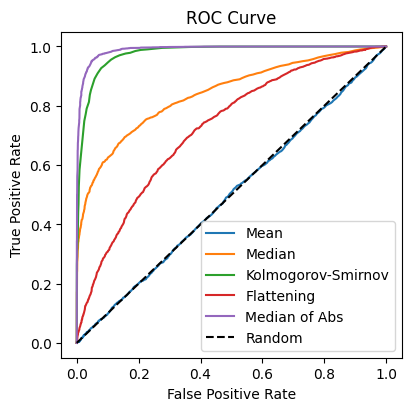
\includegraphics[width=7cm]{img/roc_curves.png}
\caption{ROC curves for different test statistics.}
\label{fig:roc}
\end{figure}

\hl{Analyser les résultats obtenus}
\hl{Ajouter la courbe de Neyman-Pearson optimale pour la comparaison comme référence théorique}

\subsection{P-value analysis}

A p-value is defined as the probability of observing a test statistic as extreme or more extreme than the observed value, assuming the null hypothesis ${\mathcal{H}}_0$ is true. Formally, for a test statistic $T$ and observed value $t_{\text{obs}}$:
\begin{equation}
p\text{-value} = P(T \geq t_{\text{obs}} | {\mathcal{H}}_0)
\end{equation}

\hl{Pour l'approche Neyman-Pearson (ou Likelihood-Ratio), il faut en faire une section à part dans la section précédente en explicitant le Likelihood-Ratio et les paramètres dont il dépend sous les 2 hypothèses, puis en tirer la statistique de test que ça donne en prenant le log etc. Expliquer aussi l'intérêt du test de Neyman-Pearson.}

\begin{figure}[H]
\centering
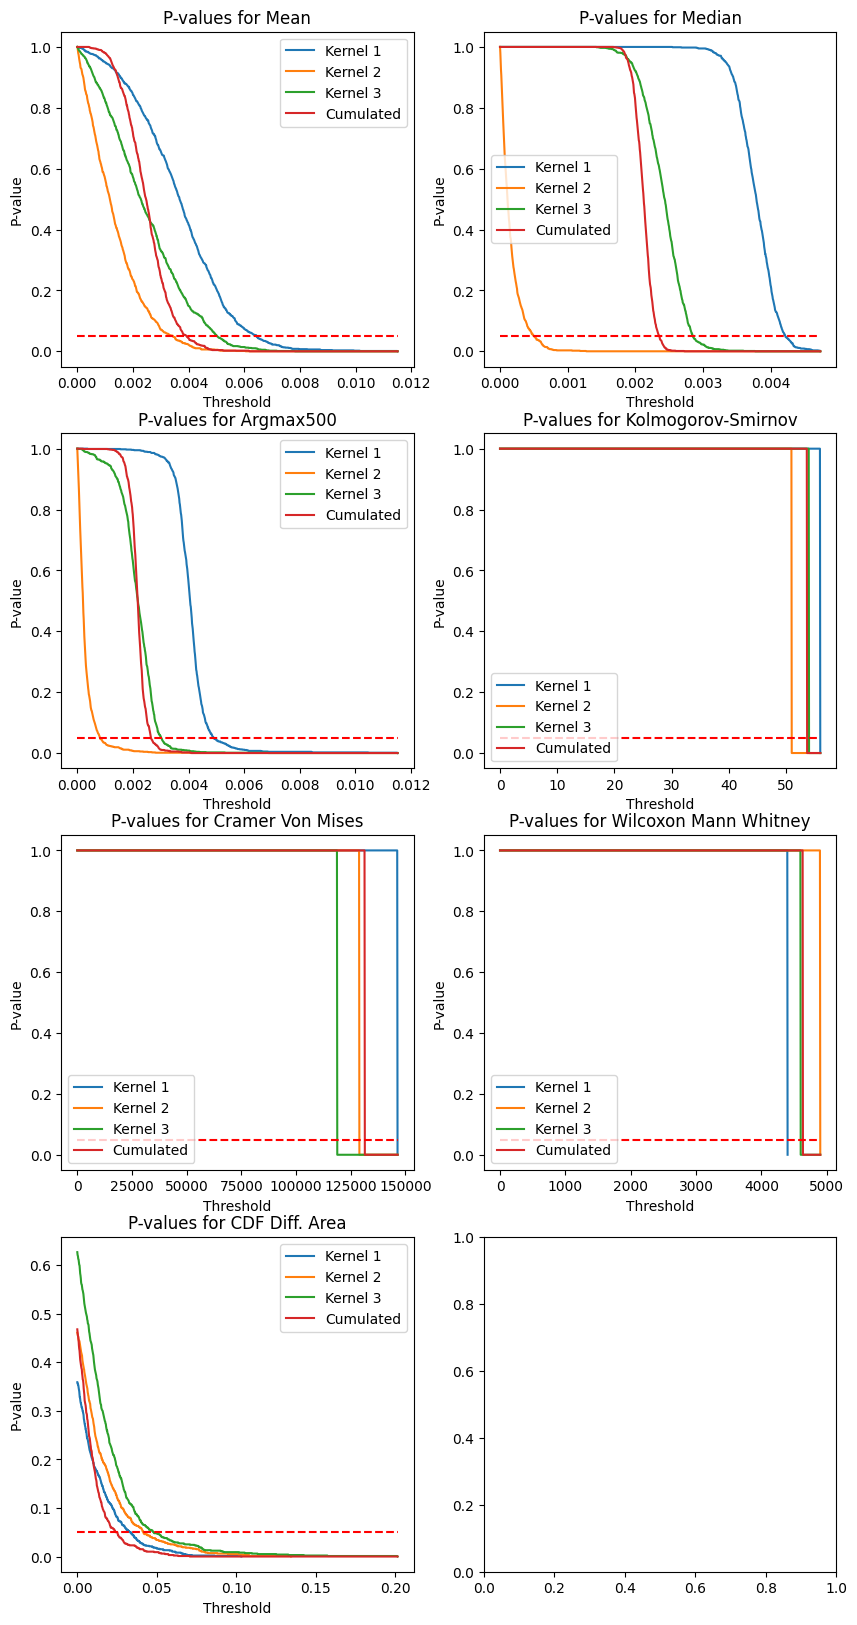
\includegraphics[width=10cm]{img/p-values.png}
\caption{Calibration of p-values for different test statistics. \hl{Cette figure doit être refaite pour se focaliser sur un seul kernel et corriger les bugs mentionnés. On peut montrer la calibration théorique p-valeur vs statistique de test et comparer à la calibration empirique pour chaque test. Attention: les p-valeurs ne dépendent pas d'un seuil, seulement des données.}}
\label{fig:pvalues}
\end{figure}

\hl{Analyser les résultats obtenus}

%--------------------------------------------------------------------

\section{Discussion}

\subsection{Comparative test performance}

\hl{ToDo}

\subsection{Noise sensitivity}

\hl{ToDo}

%-----------------------------------------------------------------

\section{Conclusions}

\hl{ToDo}

\bibliographystyle{alpha}
\bibliography{sample}

\end{document}
